\section{Circuit Boards}
\label{sec:circuit_board}
After manufacture, the chips are mounted onto small carrier boards with 0.1~inch headers. This allows people with limited surface mount technology (SMT) assembly experience to build their own demonstration boards.

The carrier fits onto the demonstration board shown in Fig.~\ref{fig:demonstration_board} which provides:
\begin{itemize}
\item USB-C for power connection,
\item \qty{1.8}{\V} and \qty{3.3}{\V} power supplies for core and IO,
\item \qty{20}{\MHz} oscillator,
\item buttons for reset and single-step clock,
\item an 8-way DIP switch for inputs,
\item a 9-way DIP switch for design selection,
\item a 7-segment LED display for the outputs,
\item headers for all IO, including 2 standard Digilent ports (PMOD),
\item a header to select internal or external clock,
\item a header to select internal or external scan chain driver,
\item a header to engage an automatic clock divider in input pin 0.
\end{itemize}

\begin{figure}[!t]
\centering
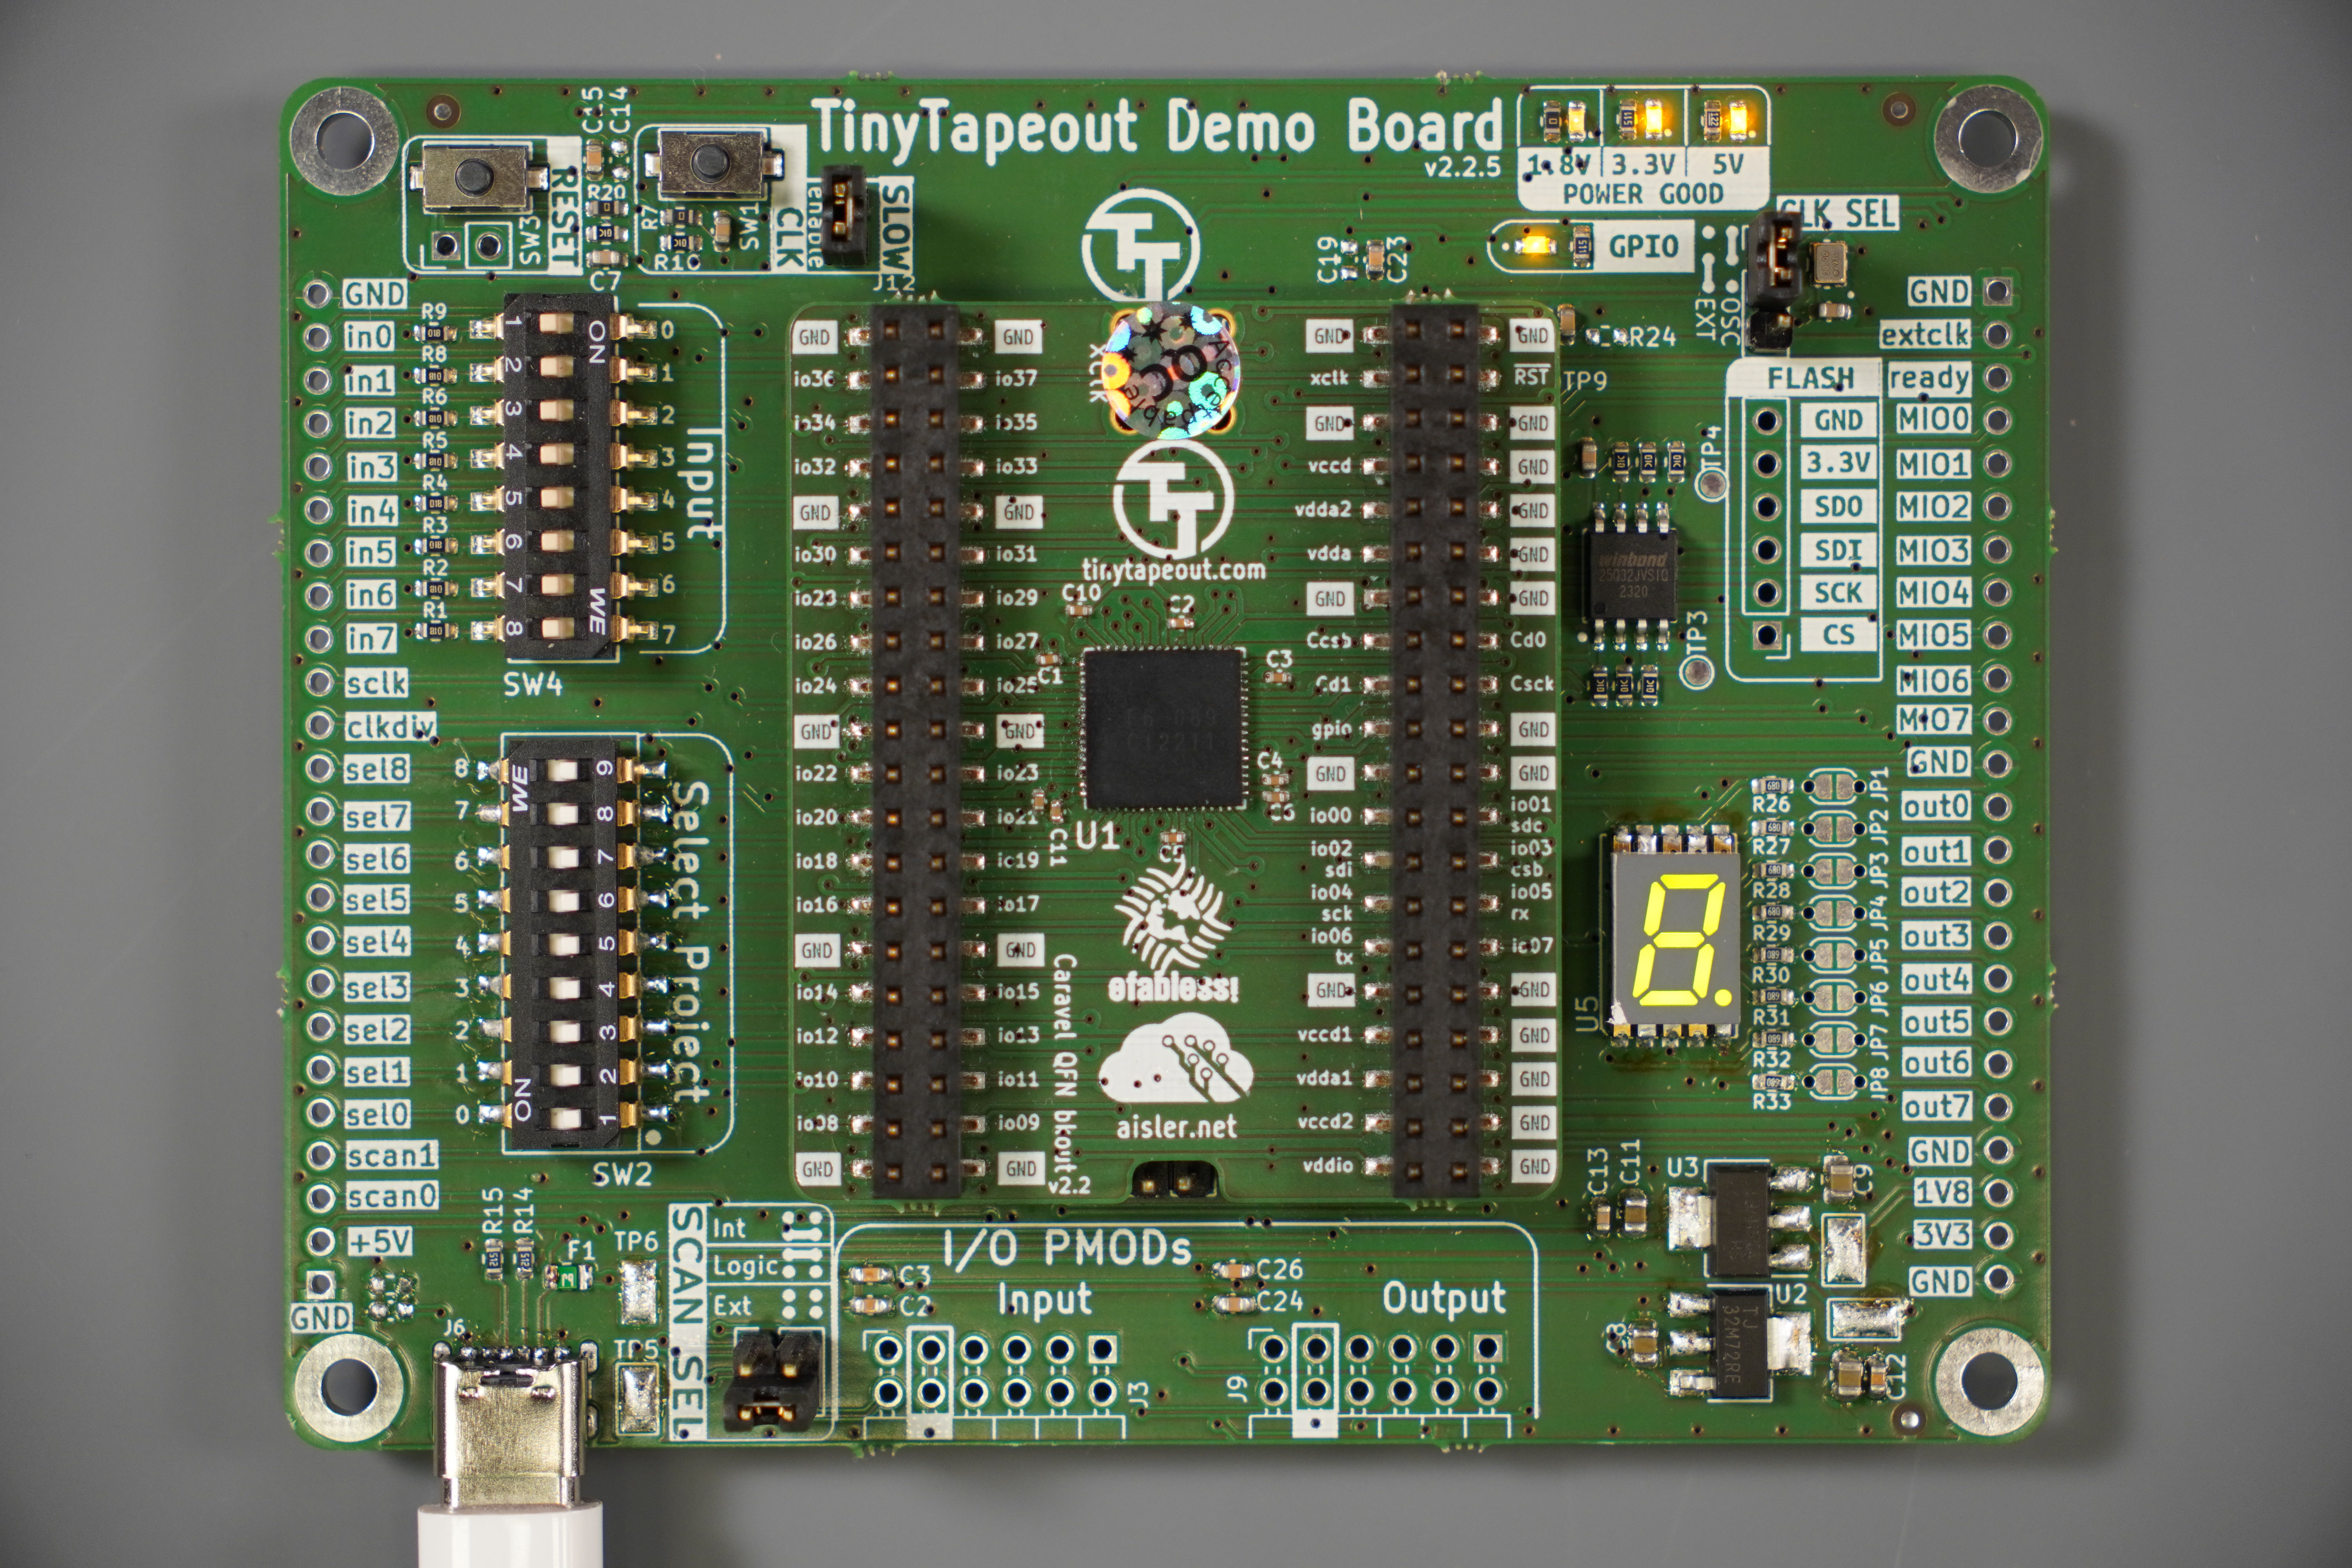
\includegraphics[width=0.5\textwidth]{./Figs/tt02 pcb assembled.JPG}
\caption{The demonstration board. Certified Open Source Hardware ES000040~\cite{oshwacertification}.}
\label{fig:demonstration_board}
\end{figure}
